\section{Transformation}

\subsection{homogene Koordinaten}

\textit{jeder Punkt P(x,y,z) des Raumes $\mathbb{R}^3$ besitzt eine 4-komponenten Vektor $\vec{r}$}
\\
$\vec{r} = \begin{bmatrix}
    x_1 \\
    x_2 \\
    x_3 \\
    x_4
\end{bmatrix}$,
$x = \frac{x_1}{x_4}$,
$y = \frac{x_2}{x_4}$,
$z = \frac{x_3}{x_4}$ \\

$(x,y,z) = (\frac{x_1}{x_4}, \frac{x_2}{x_4}, \frac{x_3}{x_4})$

\subsection{Ebene im Raum}

\textit{Ebene $\epsilon$ im Raum $\mathbb{R}^3$}
\\
$\epsilon : ax + by + cz + d = 0$
\textit{Hessische Normalform}
\\ \\
$\vec{w} = \begin{bmatrix}
    a \\
    b \\
    c \\
    d
\end{bmatrix}$, Punkt:
$\vec{r} = \begin{bmatrix}
    x \\
    y \\
    z \\
    1
\end{bmatrix}$ \\

\textit{Ebenengleichung:}

$\vec{w} \bullet \vec{r} = w^T \cdot r = ax + by + cz + d = 0$ \\

\subsection{Prokektive Transformation}

\textit{Die homogene Matrix $\mathbf{H}$ ist nur bis auf einen konstanten \
 Faktor bestimmt, heisst, alle Vielfachen von $\mathbf{H}$ sind auch gültig} \\

\text{$\eta : \mathbb{P}^3 \mapsto \mathbb{P}^3 $ stellt eine \textbf{projektiven Transformation} dar} \\

$\eta(r) = \mathbf{H} \cdot r = \begin{bmatrix}
    h_{11} & h_{12} & h_{13} & h_{14} \\
    h_{21} & h_{22} & h_{23} & h_{24} \\
    h_{31} & h_{32} & h_{33} & h_{34} \\
    h_{41} & h_{42} & h_{43} & h_{44}
\end{bmatrix} \cdot \begin{bmatrix}
    x_1 \\
    x_2 \\
    x_3 \\
    x_4
\end{bmatrix}$

\subsection{Transformationen}

$t=\begin{bmatrix}
    x \\
    y \\
    z \\
\end{bmatrix}$, $0^T = \begin{bmatrix}
    0 \\
    0 \\
    0 \\
\end{bmatrix}$, $\mathbf{RMC} =$ 3x3 Matrix

\textbf{Euklidisch} (starre Bewegung) \\
$D = \begin{bmatrix}
    \mathbf{R} & t \\
    0^T & 1
\end{bmatrix}$ \\
\textit{Abstand zwischen zwei Punkten, alle Winkel} \\
\textit{($R^{-1} = R^T$)} \\

\textbf{Ähnlichkeit} \\
$S = \begin{bmatrix}
    k \cdot \mathbf{M} & t \\
    0^T & 1
\end{bmatrix}$ \\
\textit{Winkel zwischen zwei Punkten, alle Winkel} \\

\textbf{Affin} \\
$A = \begin{bmatrix}
    \mathbf{C} & t \\
    0^T & 1
\end{bmatrix}$ \\
\textit{Parallelität, Verhältnis zwischen Volumeninhalt} \\

\textbf{Allgemein} \\
$\mathbf{H} = \begin{bmatrix}
    h_{11} & h_{12} & h_{13} & h_{14} \\
    h_{21} & h_{22} & h_{23} & h_{24} \\
    h_{31} & h_{32} & h_{33} & h_{34} \\
    h_{41} & h_{42} & h_{43} & h_{44}
\end{bmatrix}$ \\
\textit{Geraden bleiben Geraden} \\

\subsection{Translation}

$\mathbf{T}(\vec{t}) = \left[\begin{array}{ccc|c}
    1 & 0 & 0 & t_x \\
    0 & 1 & 0 & t_y \\
    0 & 1 & 0 & t_z \\
    \hline
    0 & 0 & 0 & 1 \\
\end{array}\right]$

\subsection{Rotation}

$\mathbf{R}_z = \left[\begin{array}{ccc|c}
    \cos(\Phi_z) & -\sin(\Phi_z) & 0 & 0 \\
    \sin(\Phi_z) & \cos(\Phi_z) & 0 & 0 \\
    0 & 1 & 0 & 0 \\
    \hline
    0 & 0 & 0 & 1 \\
\end{array}\right]$

$\mathbf{R}_y = \left[\begin{array}{ccc|c}
    \cos(\Phi_y) & 0 & \sin(\Phi_y) & 0 \\
    0 & 1 & 0 & 0 \\
    -\sin(\Phi_y) & 1 & \cos(\Phi_y) & 0 \\
    \hline
    0 & 0 & 0 & 1 \\
\end{array}\right]$

$\mathbf{R}_z = \left[\begin{array}{ccc|c}
    1 & 0 & 0 & 0 \\
    0 & \cos(\Phi_x) & -\sin(\Phi_x) & 0 \\
    0 & \sin(\Phi_x) & \cos(\Phi_x) & 0 \\
    \hline
    0 & 0 & 0 & 1 \\
\end{array}\right]$

\textit{Bei Rotation um selbe Achse gilt Kommutativgesetz
($\mathbf{R}_z(\Phi_{z,1} + \Phi_{z,2}) = \mathbf{R}_z(\Phi_{z,1}) \mathbf{R}_z(\Phi_{z,2}) = \mathbf{R}_z(\Phi_{z,2}) \mathbf{R}_z(\Phi_{z,1})$)}

\textit{Inverse entspricht $\mathbf{R}^{-1}(\Phi) = \mathbf{R}(-\Phi)$,
wobei $\cos(-\Phi) = \cos(\Phi)$}

\subsection{Rotation um beliebige Achse}

1) Rotation um $\phi$ um z-Achse (Matrix D) \\
2) Rotation um den Winkel $\theta \in [0, \pi]$ (um frühere X-Achse) (Matrix C)  \\
3) Rotation um den gegeben Winkel $\psi$ (Matrix B) \\

\textit{$c_\alpha = \cos \alpha$, $s_\alpha = \cos \alpha$, $\alpha \in {\phi, \theta, \psi}$} \\

\newcolumntype{C}{>{\centering\arraybackslash} m{6cm} }
\begin{tabular}{m{3cm}CC}
    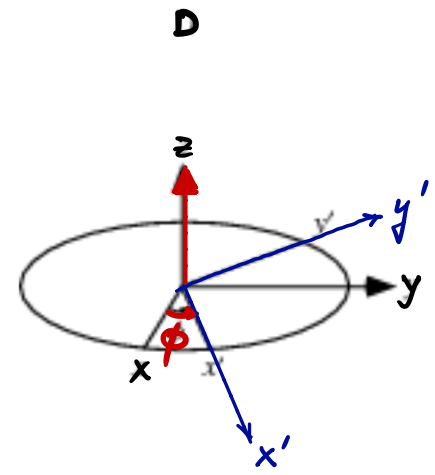
\includegraphics[scale=0.3]{rotation_matrix_D} &
    $\mathbf{D} = \begin{bmatrix}
        c_\phi & s_\phi & 0 \\
        -s_\phi & c_\phi & 0 \\
        0 & 0 & 1
    \end{bmatrix}$ \\
\end{tabular} \\
\begin{tabular}{m{3cm}CC}
    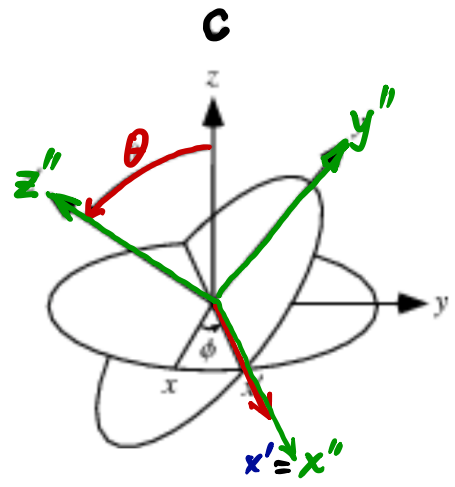
\includegraphics[scale=0.3]{rotation_matrix_C} &
    $\mathbf{C} = \begin{bmatrix}
        1 & 0 & 0 \\
        0 & c_\theta & s_\theta \\
        0 & -s_\theta & c_\theta
    \end{bmatrix}$ \\
\end{tabular} \\
\begin{tabular}{m{3cm}CC}
    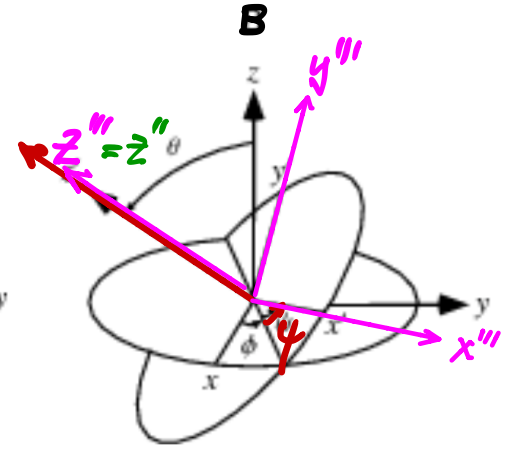
\includegraphics[scale=0.3]{rotation_matrix_B} &
    $\mathbf{B} = \begin{bmatrix}
        c_\psi & s_\psi & 0 \\
        -s_\psi & c_\psi & 0 \\
        0 & 0 & 1
    \end{bmatrix}$ \\
\end{tabular} \\

$\mathbf{M} = \mathbf{D}^{-1}\mathbf{C}^{-1}\mathbf{B}\mathbf{C}\mathbf{D}$
\textit{\\
    Bei Rotation um eine Gerade, 1. Transformation $\mathbf{D}$ \& $\mathbf{C}$
    Matrix (mit Winkel der Gerade), dann eigentliche Transformation mit gegebenem
    Winkel, dann zurücktransformiere $\mathbf{C}^{-1}$ \& $\mathbf{D}^{-1}$
}

\subsection{Rotation um eine Achse durch den Ursprung}

\textit{Rotation um einen Einheitsvektor $\vec{a} = \begin{bmatrix}
    a_1 \\
    a_2 \\
    a_3 \\
\end{bmatrix}$}

$\mathbf{Q} = (\cos \theta)I + (1-\cos \theta) \begin{bmatrix}
    a_1^2 & a_1 a_2 & a_1 a_3 \\
    a_1 a_2 & a_2^2 & a_2 a_3 \\
    a_1 a_3 & a_2 a_3 & a_3^2 \\
\end{bmatrix} -$ $\sin \theta \begin{bmatrix}
    0 & a_3 & -a_2 \\
    -a_3 & 0 & a_1 \\
    a_2 & -a_1 & 0 \\
\end{bmatrix}$

\subsection{Parallele Projektion}

\textit{Projektion auf Ebene $\epsilon: ax + by + cz + d = 0$} \\
\textit{Die Ebene ist definiert durch Normalvektor $\vec{n} = [a, b, c]^T$ (Ebenen Normalenvektor)} \\
\textit{Projektionsrichtung definiert durch Normalenvektor $\vec{v} = [v_x, v_y, v_z]^T$ (Projektionsrichtung)} \\

\begin{tabular}{cl}
    \multirow{8}{*}{
        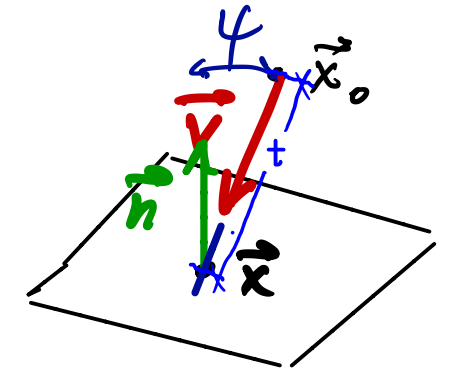
\includegraphics[width=0.2\textwidth]{assets/parallel-projection.png}
    } & $\vec{x} = \vec{x}_0 + t\vec{v} = \vec{x}_0 + t^\star\vec{v}$ \\
    & \\
    & $t = \frac{ax_0 + by_0 + cz_0 + d}{av_x + bv_y + cv_z}$\\
    & \\
    & $t = t^\star = \frac{ax_0 + by_0 + cz_0 + d}{cos(\psi)}$\\
    & \\
    & $av_x + bv_y + cv_z = \vec{v} \bullet \vec{n} =$\\
    & $|\vec{v}||\vec{n}|\cos(\psi) = \cos(\psi)$ \\
\end{tabular}

$\vec{x} = \vec{x}_0 + t\vec{v}$, komponentenweise $\begin{bmatrix}
    x = x_0 + tv_x \\
    y = y_0 + tv_y \\
    z = z_0 + tv_z \\
\end{bmatrix}$ \\
\textit{Wobei $\vec{x_0}$ Punkt dem projezierten $\vec{x}$ Punkt auf Ebene entspricht.}
\textit{$\psi$ ist der Winkel zwischen $\vec{n}$ und $\vec{v}$}

\subsection{Parallele Projektionsmatrix}

$\begin{bmatrix}
    x^* \\
    y^* \\
    z^*
\end{bmatrix} = \mathbf{H} \begin{bmatrix}
    x_0 \\
    y_0 \\
    z_0
\end{bmatrix} = $ \\
$\frac{1}{c_\psi} \begin{bmatrix}
    (c_\psi - av_x) & -bv_x & -cv_x & -dv_x \\
    -av_y & (c_\psi - bv_y) & -cv_y & -dv_y \\
    -av_z & -bv_z & (c_\psi - cv_z) & -dv_z \\
    0 & 0 & 0 & c_\psi
\end{bmatrix} \begin{bmatrix}
    x_0 \\
    y_0 \\
    z_0 \\
    1
\end{bmatrix}$ \\
\textit{$cos(\psi) = c_\psi$}

\subsection{Perspektivische Projektion}

\textit{Fall wenn Zentrum $O$ im Nullpunkt} \\

$\epsilon: ax + by + cz + d = 0$, Ebene \\

\textit{Beliebigen Punkt $A_0(x_0,y_0,z_0)$ mit Projektionspunkt $A^*(x^*,y^*,z*)$ in Ebene $\epsilon$} \\

$\begin{bmatrix}
    x^* \\
    y^* \\
    z^* \\
\end{bmatrix} = \begin{bmatrix}
    \lambda x_0 \\
    \lambda y_0 \\
    \lambda z_0
\end{bmatrix}$ \\

$\lambda = -\frac{d}{ax_0 + by_0 + cz_0}$ \\

$(ax_0 + by_0 + cz_0) \cdot \begin{bmatrix}
    x^* \\
    y^* \\
    z^* \\
    1
\end{bmatrix} = \begin{bmatrix}
    -dx_0 \\
    -dy_0 \\
    -dz_0 \\
    ax_0 + by_0 + cz_0
\end{bmatrix} = \begin{bmatrix}
    -d & 0 & 0 & 0 \\
    0 & -d & 0 & 0 \\
    0 & 0 & -d & 0 \\
    a & b & c & 0
\end{bmatrix} \begin{bmatrix}
    x_0 \\
    y_0 \\
    z_0 \\
    1
\end{bmatrix}$ \\

\subsection{Perspektivische Projektionmatrix}

$\mathbf{H} = \begin{bmatrix}
    -d & 0 & 0 & 0 \\
    0 & -d & 0 & 0 \\
    0 & 0 & -d & 0 \\
    a & b & c & 0
\end{bmatrix}$ \\

\textit{Projektionszentrum muss dann im zentrum liegen.}

\textit{\\
    Wenn Ebene nicht mit Nullpunkt im Zentrum, dann zum Zentrum transferieren.
    Wichtig, die perspektivische Ebene muss transferiert werden. Bsp: x-y-Ebene hat $\epsilon: z = 0$
    dies mit der Transformation multiplizieren. Bei Zentrum der x-y-Ebene $Z(2,4,-3)$ entspricht
    $\epsilon^\star: z = 3$, da $d = 3$ wenn 0 Punkt verschoben:
}
$[-2, -4, 3, 1] \begin{bmatrix}
    0 \\ 0 \\ 1 \\ d \\
\end{bmatrix} = 0$

\subsection{Sichtvolumen Clipping}

\textit{Das kanonische Sichtvolmen ist ein Würfel mit $P(\pm 1, \pm 1, \pm 1)$} \\
\textit{Defür sind vorne und hinten, sowie zwei Punkte bestimmend Grösse gegeben} \\

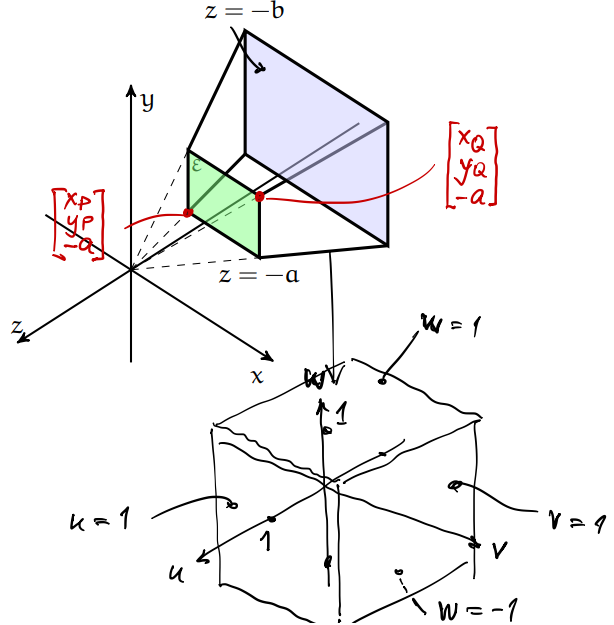
\includegraphics[scale=0.4]{clipping} \\

\textit{$P$ links unten, $Q$ rechts oben} \\
\textit{$z$ vorne $z=-a$, $z$ hinten $z=-b$} \\

$\mathbf{T} = \begin{bmatrix}
    \frac{2a}{x_Q - x_P} & 0 & \frac{x_Q + x_P}{x_Q - x_P} & 0 \\
    0 & \frac{2a}{y_Q - y_P} & \frac{y_Q + y_P}{y_Q - y_P} & 0 \\
    0 & 0 & -\frac{b+a}{b-a} & -2\frac{ba}{b-a} \\
    0 & 0 & -1 & 0 \\
\end{bmatrix}$
